% !Mode:: "TeX:UTF-8"
\chapter{First Glance of Visual SLAM}
\begin{mdframed}
	\textbf{Goal of Study}
	\begin{enumerate}[labelindent=0em,leftmargin=1.5em]
		\item Understand which modules a visual SLAM framework consists of, and what task each module carries out.
		\item Set up the programming environment, and prepare for experiments.
		\item Understand how to compile and run a program under Linux. If there is a problem, how to debug it.
		\item Learn the basic usage of cmake.
	\end{enumerate}
\end{mdframed}

\newpage
\section{Introduction}

This lecture summarizes the structure of a visual SLAM system as an outline of subsequent chapters. Practice part introduces the fundamentals of environment setup and program development. We will make a small "Hello SLAM" program at the end.

\section{Meet "Little Carrot"}

Suppose we assembled a robot called \emph{Little Carrot}, as shown in the following figure:

\begin{figure}
	\centering
	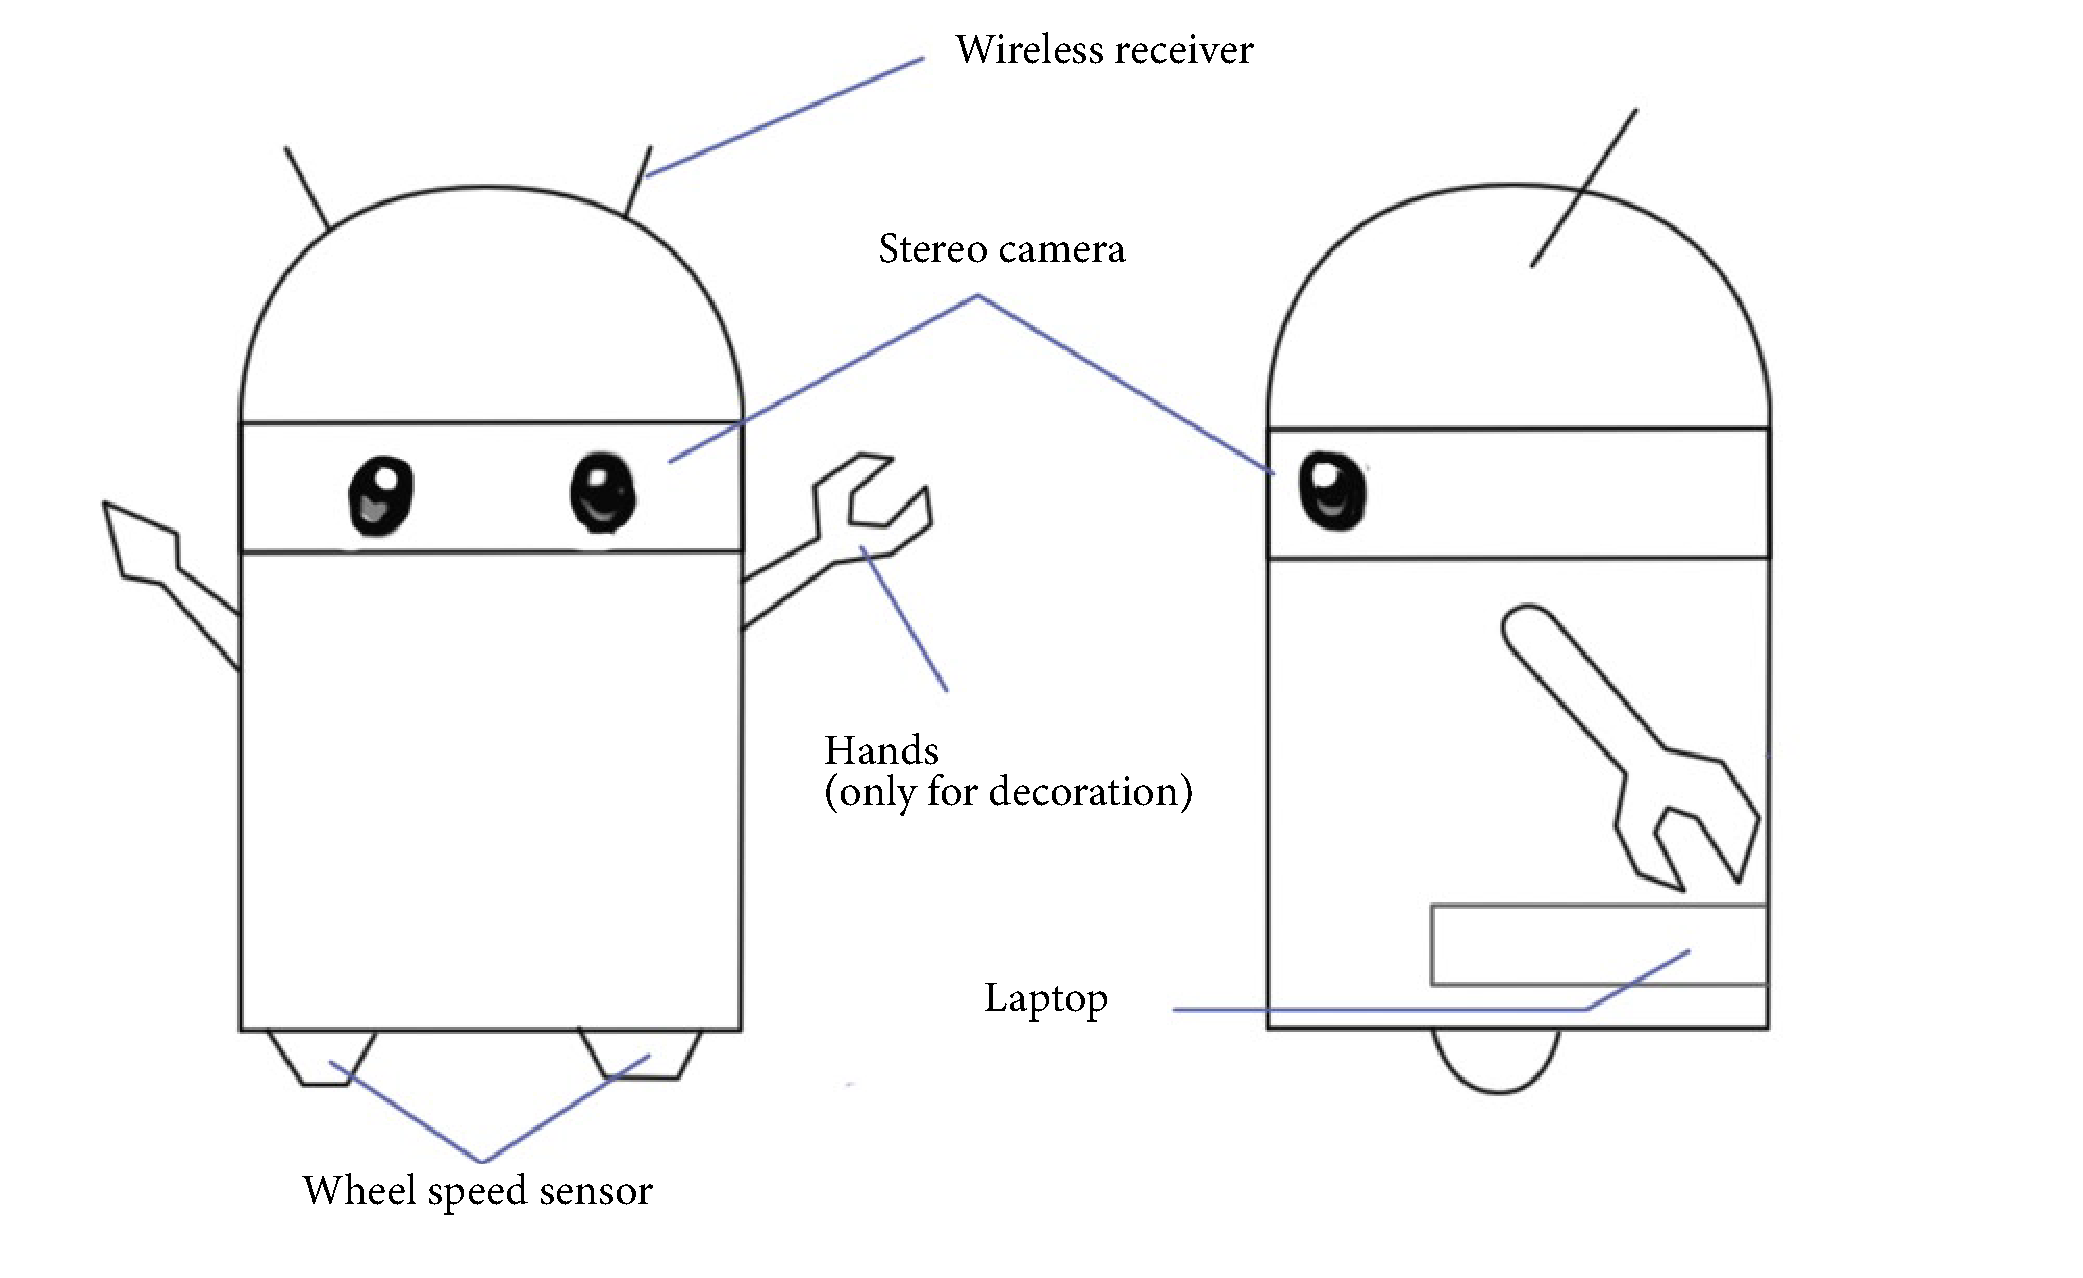
\includegraphics[width=0.8\textwidth]{resources/whatIsSLAM/carrot.pdf}
	\caption{The sketch of robot \emph{Little Carrot}}
\end{figure}

Although it looks a bit like the Android robot, it has nothing to do with the Android system. We put a laptop into its trunk (so that we can debug programs at any time). So, what is our robot capable to do?

We hope Little Carrot has the ability of \emph{autonomous moving}. Although there are many \emph{robots} placed statically on desktops, capable of chatting with people or playing music, but a tablet computer nowadays can also deliver the same tasks. As a robot, we hope Little Carrot can move freely in a room. Wherever we say hello to it, it can come to us right away.

First of all, such a robot needs wheels and motors to move, so we installed wheels under Little Carrot (gait control for humanoid robots is very complicated, which we will not be considering here). Now with the wheels, the robot is able to move, but without an effective navigation system, Little Carrot does not know where a target of action is, and it can do nothing but wander around blindly. Even worse, it may hit a wall and cause damage. In order to avoid this, we installed cameras on its head, with the intuition that such a robot \emph{should look similar to human}. Certainly, with eyes, brains and limbs, human can walk freely and explore any environment, so we (somehow naively) think that our robot should be able to achieve it too. Well, in order to make Little Carrot able to explore a room, we find it at least needs to know two things:

\begin{enumerate}
	\item  Where am I? - It's about \emph{localization}.
	\item What is the surrounding environment like? -It's about \emph{map building}.
\end{enumerate}

\emph{Localization} and \emph{map building}, can be seen as the perception in both inward and outward directions. As a completely autonomous robot, Little Carrot need not only to understand its own \emph{state} (i.e. the location), but also the external \emph{environment} (i.e. the map). Of course, there are many different approaches to solve these two problems. For example, we can lay guiding rails on the floor of the room, or paster a lot of artificial markers such as QR code pictures on the wall, or mount radio positioning devices on the table. If you are outdoor, you can also install a GNSS receiver (like the one in a cell phone or a car) on the head of Little Carrot. With these devices, can we claim that the positioning problem has been resolved? Let's categorize these sensors (see Fig.~\ref{fig:sensors}) into two classes.

\begin{figure}
	\centering
	\includegraphics[width=0.8\textwidth]{./resources/whatIsSLAM/sensors.jpg}
	\caption{Different kinds of sensors: (a) QR code (b) GNSS receiver (c) guiding rails (d) Laser range finder (e) Inertial measurement unit (f) stereo camera }
	\label{fig:sensors}
\end{figure}

The first class are \emph{non-intrusive} sensors which are completely self-contained inside a robot, such as wheel encoders, cameras, laser scanners, etc. They do not assume an cooperative environment around the robot. The other class are \emph{intrusive} sensors depending on a prepared environment, such as the above mentioned guiding rails, QR codes, etc. Intrusive sensors can usually locate a robot directly, solving the positioning problem in a simple and effective manner. However, since they require changes on the environment, the scope of usage is often limited within a certain degree. For example, if there is no GPS signal, or guiding rails cannot be laid, what should we do in those cases?

We can see that the intrusive sensors place certain \emph{constraints} to the external environment. A localization system based on them can only function properly when those constraints are met in the real world. Otherwise, the localization approach cannot be carried out anymore, like GPS positioning system normally doesn't work well in indoor environments. Therefore, although this type of sensor is simple and reliable, they do not work as a general solution. In contrast, non-intrusive sensors, such as laser scanners, cameras, wheel encoders, Inertial Measurement Units (IMUs), etc., can only observe indirect physical quantities rather than the direct locations. For example, a wheel encoder measures the wheel rotation angle, an IMU measures the angular velocity and the acceleration, a camera or a laser scanner observe the external environment in a certain form like point-clouds and images. We have to apply algorithms to infer positions from these indirect observations. While this sounds like a roundabout tactic, the more obvious benefit is that it does not make any demands on the environment, making it possible for this localization framework to be applied to an unknown environment. Therefore, they are called as self-localization in many research area.

Looking back at the SLAM definitions discussed earlier, we emphasized an \emph{unknown environment} in SLAM problems. In theory, we should not presume which environment the Little Carrot will be used (but in reality we will have a rough range, such as indoor or outdoor), which means that we can not assume that the external sensors like GPS can work smoothly. Therefore, the use of portable non-intrusive sensors to achieve SLAM is our main focus. In particular, when talking about visual SLAM, we generally refer to the using of \emph{cameras} to solve the localization and map building problems.

Visual SLAM is the main subject of this book, so we are particularly interested in what the Little Carrot's eyes can do. The cameras used in SLAM are different from the commonly seen SLR cameras. It is often much simpler and does not carry expensive lens. It shoots at the surrounding environment at a certain rate, forming a continuous video stream. An ordinary camera can capture images at 30 frames per second, while high-speed cameras can do faster. The camera can be roughly divided into three categories: Monocular, Stereo and RGB-D, as shown by the following figure \ref{fig:cameras}. Intuitively, a monocular camera has only one camera, a stereo camera has two. The principle of a RGB-D camera is more complex, in addition to being able to collect color images, it can also measure the distance of the scene from the camera for each pixel. RGB-D cameras usually carry multiple cameras, and may adopt a variety of different working principles. In the fifth lecture, we will detail their working principles, and readers just need an intuitive impression for now. In addition, there are also specialty and emerging camera types can be applied to SLAM, such as panorama camera \cite{Pretto2011}, event camera \cite{Rueckauer2016}. Although they are occasionally seen in SLAM applications, so far they have not become the mainstream. From the appearance we can infer that Little Carrot seems to carry a stereo camera.

\begin{figure}
	\centering
	\includegraphics[width=0.8\textwidth]{./resources/whatIsSLAM/camera.pdf}
	\caption{Different kinds of cameras: monocular, RGB-D and stereo. }
	\label{fig:cameras}
\end{figure}

Now, let's take a look at the pros and cons of using different type of camera for SLAM.

\subsubsection{Monocular Camera}

The SLAM system that uses only one camera is called Monocular SLAM. This sensor structure is particularly simple, and the cost is particularly low, therefore the monocular SLAM has been very attractive to researchers. You must have seen the output data of a monocular camera: photo. Yes, as a photo, what are its characteristics?

A photo is essentially a \emph{projection} of a scene onto a camera's imaging plane. It reflects a three-dimensional world in a two-dimensional form. Obviously, there is one dimension lost during this projection process, which is the so-called depth (or distance). In a monocular case, we can not obtain the \emph{distance} between objects in the scene and the camera by using a single image. Later we will see that this distance is actually critical for SLAM. Because we human have seen a large number of images, we formed a natural sense of distances for most scenes, and this can help us determine the distance relationship among the objects in the image. For example, we can recognize objects in the image and correlate them with their approximate size obtained from daily experience. The close objects will occlude the distant objects; the sun, the moon and other celestial objects are infinitely far away; an object will have shadow if it is under sunlight. This common sense can help us determine the distance of objects, but there are also certain cases that confuse us, and we can no longer determine the distance and true size of an object. The following figure \ref{fig:why-depth} is shown as an example. In this image, we can not determine whether the figures are real person or small toys purely based on the image itself. Unless we change our view angle, explore the three-dimensional structure of the scene. In other words, from a single image, we can not determine the true size of an object. It may be a big but far away object, but it may also be a close but small object. They may appear to be the same size in an image due to the perspective projection effect.

\begin{figure}
	\centering
	\includegraphics[width=0.8\textwidth]{./resources/whatIsSLAM/why-depth.pdf}
	\caption{We cannot tell if the people are real humans or just small toys from a single image}
	\label{fig:why-depth}
\end{figure}

Since the image taken by an monocular camera is just a 2D projection of the 3D space, if we want to recover the 3D structure, we have to change the camera's view angle. Monocular SLAM adopts the same principle. We move the camera and estimate its own \emph{motion}, as well as the distances and sizes of the objects in the scene, namely the \emph{structure} of the scene. So how should we estimate these movements and structures? From the everyday experience we know that if a camera moves to the right, the objects in the image will move to the left which gives us an inspiration of inferring motion. On the other hand, we also know that closer objects move faster, while distant objects move slower. Thus, when the camera moves, the movement of these objects on the image forms pixel disparity. Through calculating the disparity, we can quantitatively determine which objects are far away and which objects are close.

However, even if we know which objects are near and which are far, they are still only relative values. For example, when we are watching a movie, we can tell which objects in the movie scene are bigger than the others, but we can not determine the \emph{real size} of those objects -- are the buildings real high-rise buildings or just models on a table? Is it a real monster that destructs a building, or just an actor wearing special clothing? Intuitively, if the camera's movement and the scene size are doubled at the same time, monocular cameras see the same. Likewise, multiplying this size by any factor, we will still get the same picture. This demonstrates that the trajectory and map obtained from monocular SLAM estimation will differ from the actual trajectory and map with a factor, which is just the so-called \emph{scale} \footnote{Mathematical reason will be explained in the visual odometry chapter.}. Since monocular SLAM can not determine this real scale purely based on images, this is also called the \emph{scale ambiguity}.

In monocular SLAM, depth can only be calculated with translational movement, and the real scale cannot be determined. These two things could cause significant trouble when applying monocular SLAM into real-world applications. The fundamental cause is that depth can not be determined from a single image. So, in order to obtain real-scaled depth, we start to use stereo and RGB-D cameras.

\subsubsection{Stereo Camera and RGB-D Camera}
The purpose of using stereo and RGB-D cameras is to measure the distance between objects and the camera, to overcome the shortcomings of monocular cameras that distances are unknown. Once distances are known, the 3D structure of a scene can be recovered from a single frame, and also eliminates the scale ambiguity. Although both stereo and RGB-D cameras are able to measure the distance, their principles are not the same. A stereo camera consists of two synchronized monocular cameras, displaced with a known distance, namely the \emph{baseline}. Because the physical distance of the baseline is know, we are able to calculate the 3D position of each pixel, in a way that is very similar to our human eyes. We can estimate the distances of the objects based on the differences between the images from left and right eye, and we can try to do the same on computers (see Fig.~\ref{fig:stereo}). We can also extend stereo camera to multi-camera systems if needed, but basically there is no much difference.

\begin{figure}
    \centering
    \includegraphics[width=0.8\textwidth]{./resources/whatIsSLAM/stereo.pdf}
    \caption{Distance is calculated from the disparity of two stereo image pair.}
    \label{fig:stereo}
\end{figure}


Stereo cameras usually require significant amount of computational power to (unreliably) estimate depth for each pixel. This is really clumsy compared to human beings. The depth range measured by a stereo camera is related to the baseline length. The longer a baseline is, the farther it can measure. So stereo cameras mounted on autonomous vehicles are usually quite big. Depth estimation for stereo cameras is achieved by comparing images from the left and right cameras, and does not rely on other sensing equipment. Thus stereo cameras can be applied both indoor and outdoor. The disadvantage of stereo cameras or multi-camera systems is that the configuration and calibration process is complicated, and their depth range and accuracy are limited by baseline length and camera resolution. Moreover, stereo matching and disparity calculation also consumes much computational resource, and usually requires GPU or FPGA to accelerate in order to generate real-time depth maps. Therefore, in most of the state-of-the-art algorithms, computational cost is still one of the major problems of stereo cameras.

Depth camera (also known as RGB-D camera, RGB-D will be used in this book) is a type of new cameras rising since 2010. Similar to laser scanners, RGB-D cameras adopt infrared structure of light or Time-of-Flight (ToF) principles, and measure the distance between objects and the camera by actively emitting light to the object and receive the returned light. This part is not solved by software as a stereo camera, but by physical sensors, so it can save much computational resource compared to stereo cameras (see Fig.~\ref{fig:RGBD}). Common RGB-D cameras include Kinect / Kinect V2, Xtion Pro Live, RealSense, etc. However, most of the RGB-D cameras still suffer from issues including narrow measurement range, noisy data, small field of view, susceptible to sunlight interference, and unable to measure transparent material. For SLAM purpose, RGB-D cameras are mainly used in indoor environments, and are not suitable for outdoor applications.
\begin{figure}
    \centering
    \includegraphics[width=0.8\textwidth]{./resources/whatIsSLAM/rgbd.pdf}
    \caption{RGBD.}
    \label{fig:RGBD cameras measurement the distance and can build a point cloud with a single image frame.}
\end{figure}

We have discussed the common types of cameras, and we believe you should have gained an intuitive understanding of them. Now, imagine a camera is moving in a scene, we will get a series of continuously changing images \footnote{You can try to use your phone to record a video clip.}. The goal of visual SLAM is to localize and build a map using these images. This is not as simple task as you would think. It is not a single algorithm that continuously output positions and map information as long as we feed it with input data. SLAM requires a good algorithm framework, and after decades of hard work by researchers, the framework has been matured in recent years.

\section{The Classic Visual SLAM Framework}
%
%Let's take a look at the classic visual SLAM framework, shown in the following figure [workflow]:
%
%![workflow](/resources/whatIsSLAM/workflow.jpg)
%
%The entire visual SLAM work-flow includes the following steps:
%
%1.  Sensor data acquisition. In visual SLAM, this mainly refers to for acquisition and preprocessing for camera images. For a mobile robot, this will also include the acquisition and synchronization for motor encoders, IMU sensors, etc.
%2.  **Visual Odometer** (VO). The task of VO is to estimate the camera movement between adjacent frames, as well as to generate a local map. VO is also known as the **Front End**.
%3. **Backend optimization**. The back end receives camera poses at different time stamps from VO, as well as results from loop detection, and apply optimization to generate a globally consistent trajectory and map. Because it is connected after the VO, it is also known as the **Back End**.
%4. **Loop Closing**. Loop closing determines whether the robot has returned to its previous position. If a loop is detected, it will provide information to the back end for further optimization.
%5. **Mapping**. It constructs a task specific map based on the estimated camera trajectory.
%
%The classic visual SLAM framework is the result of more than a decade's research endeavor. The framework itself and the algorithms it contains have been basically finalized and have been provided in several vision and robotics libraries. Relying on these algorithms, we are able to build visual SLAM systems performing real-time positioning and mapping in normal environments. Therefore, we can draw the conclusion: **if the working environment is limited to static and rigid, with insignificant lighting changes and no human interference**, visual SLAM technology is mature [Cadena2016].
%
%The readers may have not understood the concepts of the modules yet, so we will detail the functionality of each module as follows. However, an deeper understanding of their working principles requires certain mathematical knowledge, and they will be expanded in the second part of this book. For now, an intuitive and qualitative understanding of each module is good enough.
%
%#### Visual Odometer
%
%The visual odometer is concerned with the movement of a camera between **adjacent image frames**, and the simplest case is of course the motion relationship between two successive images. For example, when we see figure [cameramotion], we will naturally reflect that the right image should be the result of the left image after a rotation to the left with a certain angle (you will feel more natural if shown in video form). Let's consider this question: how do we know the motion is "turning left"? Humans have long been accustomed to using our eyes to explore the world, and estimating our own positions, but this intuition is often difficult to explain, especially in rational language. When we see [cameramotion], we will naturally think that the bar is close to us, and the walls and the blackboard are farther away. When the camera turns to left, the closer part of the bar started to appear, and the cabinet on the right side started to move out of our sight. With this information, we conclude that the camera should be be rotating to the left.
%
%![cameramotion](/resources/whatIsSLAM/cameramotion.jpg)
%
%But if we further ask: can we determine how much the camera has rotated and translated, in units of degrees or centimeters? It is still difficult for us to give an quantitative answer. Because our intuition is not good at calculating numbers. But for a computer, movements have to be described with numbers. So we will ask: **how should a computer determine a camera's motion based on images?**
%
%As mentioned earlier, in the field of computer vision, a task that seems natural to a human can be very challenging for a computer. Images are nothing but numerical matrices in computers. A computer has no idea what these matrices mean (this is the problem that machine learning is also trying to solve). In visual SLAM, we can only see blocks of pixels, knowing that they are the results of projections by spatial points onto the camera's imaging plane. In order to quantify a camera's movement, we must first **understand the geometric relationship between a camera and the spatial points**.
%
%Some background knowledge is needed to clarify this geometric relationship and the realization of VO methods. Here we only want to convey an intuitive concept. For now, you just need to take away that VO is able to estimate camera motions from images of adjacent frames and restore the 3D structures of the scene. It is named as an "odometer", because similar to an actual odometer, it only calculates the movement at neighboring moments, and does not consider the information in the further past. In this regard, VO is like a species with only a short memory.
%
%Now, assuming that we have a visual odometer, we are able to estimate camera movements between every two successive frames. If we connect the adjacent movements, this constitutes the movement of the robot trajectory, and therefore addresses the positioning problem. On the other hand, we can calculate the 3D position for each pixel according to the camera position at each time step, and they will form an map. Up to here, it seems with an VO, the SLAM problem is already solved. Or, is it?
%
%Visual odometer is indeed an key to solving visual SLAM, we will be spending a great part to explain it in details. However, using only a VO to estimate trajectories will inevitably cause **accumulative drift**. This is due to the fact that the visual odometer (in the simplest case) only estimates the movement between two frames. We know that each estimate is accompanied by a certain error, and because the way odometers work, errors from previous moments will be carried forward to the following moments, resulting in inaccurate estimation after a period of time (see figure [loopclosure]). For example, the robot first turns left ![](http://latex.codecogs.com/gif.latex?90^\\circ) and then turns right ![](http://latex.codecogs.com/gif.latex?90^\\circ). Due to error, we estimate the first ![](http://latex.codecogs.com/gif.latex?90^\\circ) as ![](http://latex.codecogs.com/gif.latex?89^\\circ). Then we will be embarrassed to find that after the right turn, the estimated position of the robot will not return to the origin. What's worse, even the following estimates are accurate, they will always be carrying the ![](http://latex.codecogs.com/gif.latex?1^\\circ) error compared to the ground-truth.
%
%![cameramotion](/resources/whatIsSLAM/loopclosure.jpg)
%
%This is the so-called **drift**. It will cause us unable to build a consistent map. You will find the original straight corridor oblique, and the original ![](http://latex.codecogs.com/gif.latex?90^\\circ) angle crooked - this is really an unbearable thing! In order to solve the drifting problem, we also need other two components: **back-end optimization** (footnote: usually know as the back end. Since it is often the optimization methods that's used in this part, it is also called back-end optimization.) and **loop closing**. Loop closing is responsible for detecting when a robot returns to its previous position, while the back-end optimization corrects the shape of the entire trajectory based on this information.
%
%#### Back-end Optimization
%
%Generally speaking, back-end optimization mainly refers to the process of dealing with **noise** in SLAM systems. We wish that all the sensor data is accurate, but in reality, even the most high-end sensors still have certain amount of noise. Cheap sensors usually have bigger measurement errors, while that of expensive ones may be small. Moreover, performance of many sensors are affected by changes in magnetic field, temperature, etc. Therefore, in addition to solving the problem of estimating camera movements from images, we also care about how much noise this estimation contains, how these noise is carried forward from the last time step to the next, and how much confidence we have on the current estimation. So the problem that back-end optimization solves can be summarized as: to estimate the state of the entire system from noisy data and how uncertain these estimations are. This is the so-called Maximum-a-Posteriori (MAP) Estimation. The state here includes both the robot's own trajectory and the environment map.
%
%In contrast, the visual odometer part is usually referred to as the "front end". In a SLAM framework, the front end provides data to be optimized by the back end, as well as initial values 鈥嬧€媐or non-linear optimization. While the back end is responsible for the overall optimization, it often only care about the data itself, instead of what sensor the data is generated from. **In visual SLAM, the front end is more relevant to computer vision research, such as image feature extraction and matching, while the back end contains mainly filtering and nonlinear optimization algorithms.**
%
%Historically, the back-end optimization part has been equivalent to "SLAM research" for a long time. The early days, SLAM problem was described as a state estimation problem, which is exactly what the back-end optimization tries to solve. In the earliest papers on SLAM, researchers at that time called it "estimation of spatial uncertainty" [Smith1980, Smith1990]. Although it sounds obscure, it does reflect the nature of the SLAM problem: **the estimation of the uncertainty of the self-movement and the surrounding environment**. In order to solve the SLAM problem, we need state estimation theory to express the uncertainty of localization and map construction, and then use filters or nonlinear optimization to estimate the mean and uncertainty (co-variance) of the states. The details of state estimation and non-linear optimization will be described in Chapter 6, 10 and 11. Let's skip it for now.
%
%#### Loop Closing
%
%Loop Closing, also known as Loop Closure Detection, is mainly to address the drifting problem of position estimation in SLAM. How to solve it? Assuming that a robot has returned to its origin after a period of movement, but the estimated position does not return to the origin due to drift. How to correct it? Imagine that if there is some way to let the robot know that it has returned to the origin, or the "origin" can be identified again, we can then "pull" the estimated locations to the origin to eliminate drifts. This process is called loop closing.
%
%Loop closing has close relationship with both "positioning" and "map building". In fact, the main purpose of building a map is to enable a robot to know places it has been to. In order to achieve loop closing, we need to let the robot has the ability to identify the scenes it has visited before. There are different alternatives to achieve this goal. For example, as we mentioned earlier, we can set a marker at where the robot starts, such as a QR code. If it sees the sign again, we know that it has returned to the origin. However, the marker is essentially an intrusive sensor, it sets constraints to the application environment (what if putting up QR code is not allowed?). We will prefer the robot can use its non-intrusive sensors, e.g. the image itself, to complete this task. One possible approach would be to detect similarities between images. This is inspired by us humans. When we see two similar images, it is easy to identify that they are taken from the same place. If the loop closing is successful, accumulative error can be significantly reduced. Therefore, visual loop detection is essentially an algorithm for calculating similarities of images. The rich information contained in images can remarkably reduce the difficulty of making correct loop detection.
%
%After a loop is detected, we will tell the back-end optimization algorithm that "A and B are the same point". Then, based on this new information, the trajectory and the map will be adjusted to match the loop detection result. In this way, if we have sufficient and reliable loop detection, we can eliminate cumulative errors, and get globally consistent trajectories and maps.
%
%#### Mapping
%
%Mapping refers to the process of building a map. A map (see figure [map]) is a description of the environment, but the way of describing is not fixed and depends on the actual application.
%
%![map](/resources/whatIsSLAM/map.jpg)
%
%For home sweeping robots, since they mainly move on ground, a two-dimensional map with marks for open areas and obstacles would be sufficient for navigation to a certain extend. And for a camera, we need at least a three-dimensional map for its 6 degrees of freedom movement. Sometimes, we want a beautiful reconstruction result, not just a set of points, but also with texture of triangular facets. At other times, we do not care about the map, just need to know things like "point A and point B are connect, while point B and point C are not". Sometimes maps may not even be needed, or they are available from others, for example, driving vehicles can often obtain local maps plotted by others.
%
%For maps, we have so many ideas and demands. So compared to the previously mentioned visual odometer, loop closure detection and back-end optimization, map building does not refer to a fixed form or algorithm. A collection of spatial points can be called a map, a beautiful 3D model is also a map, so is a picture of a city, a village, railways, and rivers. The form of the map depends on the application of SLAM. In general, they can be divided into to categories: **metric map** and **topological map**.
%
%##### Metric Map
%
%Metric maps emphasize the exact locations of objects in maps, are usually classified as either sparse or dense. Sparse metric maps abstract a scene into certain form, and do not express all the objects. For example, we can construct a sparse map by selecting representative landmarks such as road signs, and ignore other parts. In contrast, dense metric maps focus on modeling all the things that are seen. For positioning, sparse map is enough, while for navigation, a dense map is usually needed (otherwise we may hit a wall between two road signs). A dense map usually consists of a number of small pieces at a certain resolution. It can be small grids for 2D metric maps, or small voxels for 3D. Usually, a small piece may have three states to express whether an object is there: occupied, idle, and unknown. When a spatial location is queried, the map can give information about whether the location can be passed through. This type of maps can be used for a variety of navigation algorithms, such as A\*, D\* (footnote: [https://en.wikipedia.org/wiki/A*_search_algorithm](https://en.wikipedia.org/wiki/A*_search_algorithm)), etc., and thus attracts the attention of researchers in robotics field. But we can also see that this map needs to store the state of each grid, and thus being storage expensive. Even worse, in most cases, a large portion of the map details is useless. On the other hand, there is sometimes a consistency issue with large-scale metric maps. A little bit of steering error may cause the walls of two rooms to overlap and thus making the map ineffective.
%
%##### Topological Map
%
%Compared to the accurate metric maps, topological maps emphasize the relationships among map elements. A topological map is a graph composed of nodes and edges, only considering the connectivity between nodes. For instance, we only care about that point A and point B are connected, regardless how we could travel from point A to point B. It relaxes the requirements on precise locations of a map by removing map details, and is therefore a more compact expression. However, topological maps are not good at representing maps with complex structures. Questions such as how to split a map to form nodes and edges, and how to use a topological map for navigation and path planning, are still open problems to be studied.
%
%### Mathematical Formulation of SLAM Problems
%
%Through the previous introduction, readers should have gained an intuitive understanding of the modular composition of a SLAM system and the main functionality of each module. However, we cannot write runable programs only based on intuitive impressions. We want to rise it to a rational and rigorous level, that is, using mathematical language to formulate a SLAM process. We will be using variables and formulas, but please rest assured that we will try our best to keep it clear enough.
%
%Assuming that our Little Carrot is moving in an unknown environment, carrying some sensors. How can this be described in mathematical language? First, since sensors usually collect data at different some points, we are only concerned with the locations and map at these moments. This turns a continuous period of time into discrete time steps ![](http://latex.codecogs.com/gif.latex?t=1,\\cdots,K), at which data sampling happens. We use ![](http://latex.codecogs.com/gif.latex?\\bm{x}) to indicate positions of Little Carrot. So the positions at different time steps can be written as ![](http://latex.codecogs.com/gif.latex?\\bm{x}_1,\\cdots,\\bm{x}_K), which constitute the trajectory of Little Carrot. In terms of the map, we assume that the map is made up of a number of **landmark**, and at each time step, the sensors can see a portion of the landmarks and record their observations. Assume there are in total ![](http://latex.codecogs.com/gif.latex?N) landmarks, and we will use ![](http://latex.codecogs.com/gif.latex?\\bm{y}_1,\\cdots,\\bm{y}_N) to represent them.
%
%With such a setting, "Little Carrot move in the environment with sensors" have two aspects to be described:
%
%1.  What is its **motion**? We want to describe how ![](http://latex.codecogs.com/gif.latex?\\bm{x}) is changed from time step ![](http://latex.codecogs.com/gif.latex?k-1) to ![](http://latex.codecogs.com/gif.latex?k).
%2.  What are the **observations**? Assuming that the Little Carrot detects a certain landmark ![](http://latex.codecogs.com/gif.latex?\\bm{y}_j) at position ![](http://latex.codecogs.com/gif.latex?\\bm{x}_k) with a time stamp ![](http://latex.codecogs.com/gif.latex?k), we need to describe this event in mathematical language.
%
%Let's first take a look at motion. Typically, a robot always carries certain kind of sensors to measure its own movement, such as an encoder or inertial sensor. These sensors can measure readings regarding its motion, but not necessarily directly the location difference. Instead, readings could be acceleration, angular velocity and other information. However, no matter what the sensor is, we can use a common and abstract mathematical model to describe it:
%
%![](http://latex.codecogs.com/gif.latex?\\bm{x}_k=f\\left({{\\bm{x}_{k-1}},{\\bm{u}_k},\\bm{w}_k}\\right))
%
%Where ![](http://latex.codecogs.com/gif.latex?\\bm{u}_k) is the motion sensor reading (sometimes called the **input**), while ![](http://latex.codecogs.com/gif.latex?\\bm{w}_k) is noise. Note that we use a general function ![](http://latex.codecogs.com/gif.latex?f) to describe the process, instead of specifying the way ![](http://latex.codecogs.com/gif.latex?f) works. This allows the function to represent any motion sensor, rather than being limited to a particular one, and thus becoming a general equation, . We call it the **motion equation**.
%
%Corresponding to the motion equation, there is also a **observation equation**. The observation equation describes that when the Little Carrot sees a landmark point ![](http://latex.codecogs.com/gif.latex?\\bm{y}_j) at ![](http://latex.codecogs.com/gif.latex?\\bm{x}_k) and generates an observation data ![](http://latex.codecogs.com/gif.latex?\\bm{z}_{k,j}). Likewise, we will describe this relationship with an abstract function ![](http://latex.codecogs.com/gif.latex?h):
%
%![](http://latex.codecogs.com/gif.latex?\\bm{z}_{k,j}=h\\left({{\\bm{y}_j},{\\bm{x}_k},\\bm{v}_{k,j}}\\right))
%
%Where, ![](http://latex.codecogs.com/gif.latex?\\bm{v}_{k,j}) is the noise in this observation. Since there are more forms of observation sensors, the observed data ![](http://latex.codecogs.com/gif.latex?\\bm{z}) and the observed equation ![](http://latex.codecogs.com/gif.latex?h) also have many different forms.
%
%Readers may wonder that the function ![](http://latex.codecogs.com/gif.latex?f,h) we used do not seem to specify what the motion and observations exactly are. Besides, what are ![](http://latex.codecogs.com/gif.latex?\\bm{x}), ![](http://latex.codecogs.com/gif.latex?\\bm{y}), ![](http://latex.codecogs.com/gif.latex?\\bm{z}) here? In fact, according to the actual movement of Little Carrot and the type of sensor it carries, there are different ways for **parameterization**. What is parameterization then? For example, suppose the Little Carrot moves in a plane, then its pose (footnote: In this book, we use the word "pose" to refer to "position" plus "orientation".) is described by two position values and one angle, i.e. ![](http://latex.codecogs.com/gif.latex?\\bm{x}_k=[x,y,\theta]_k^\mathrm{T}). At the same time, the motion sensor can measure the amount of change in the position and angle of Little Carrot at any time step interval ![](http://latex.codecogs.com/gif.latex?\\bm{u}_k=[\\Delta{x},\\Delta{y},\\Delta\\theta]_k^\\mathrm{T}). Then, the motion equation can be specified as 
%
%![](http://latex.codecogs.com/gif.latex?{\\left[\\begin{array}{l}x\\\y\\\\\theta\\end{array}\\right]_k}={\\left[\\begin{array}{l}x\\\y\\\\\theta\\end{array}\\right]_{k-1}}+{\\left[\\begin{array}{l}\\Delta{x}\\\\\Delta{y}\\\\\Delta\\theta\\end{array}\\right]_k}+w_k)
%
%This is a simple linear relationship. However, not all of the sensors can directly measure the displacement and angle changes, so there are other forms of more complex equations of motion, then we may need to carry out dynamic analysis. On the observation equation, for example, a small radish carrying a two-dimensional laser sensor. We know that when a laser sensor observes a 2D punctuation, two quantities can be measured: the distance between the road sign and the radish body is $ r $ and the angle $$ \ phi $$. The observation data is $ \ bm {y} = [p_x, p_y] ^ \ mathrm {T} $ (for the sake of simplicity, omitting the subscript), the observation data is $ \ bm {z} = [r, \ phi] ^ \ Mathrm {T} $, then the observation equation is as follows: